\subsection{Granularity}
The granularity of a \textit{task} is defined by the lecturer (or creator of the task). At the coarsest granularity in the context of, for example, exercise sheets, a \textit{task} should reflect one exercise sheet. Of course a finer level of granularity can be chosen. In the context of exercise sheets this could mean, that there is one \textit{task} per task on an exercise sheet. Ultimately it is the lecturers responsibility to communicate the granularity of the \textit{task}.

\subsection{Process of Task Creation}
The process of \textit{task creation} is designed in a linear fashion. There are four consecutive steps involved in \textit{task creation}.

\begin{enumerate}
  \item Entering general information. Part of the \nameref{sub:metainfo}.
  \item Selecting a main topic. Part of the \nameref{sub:metainfo}.
  \item Selecting \nameref{sub:features} with their associated \textit{weights}.
  \item Overviewing and validating the choices made in the previous steps. 
\end{enumerate}

In order to get to the next/previous step the user can press the \textit{BACK}-/\textit{NEXT}-Buttons (labeled 9 and 10 in Figure~\ref{fig:taskcreation1}).

\begin{figure}[h]
  \begin{center}
    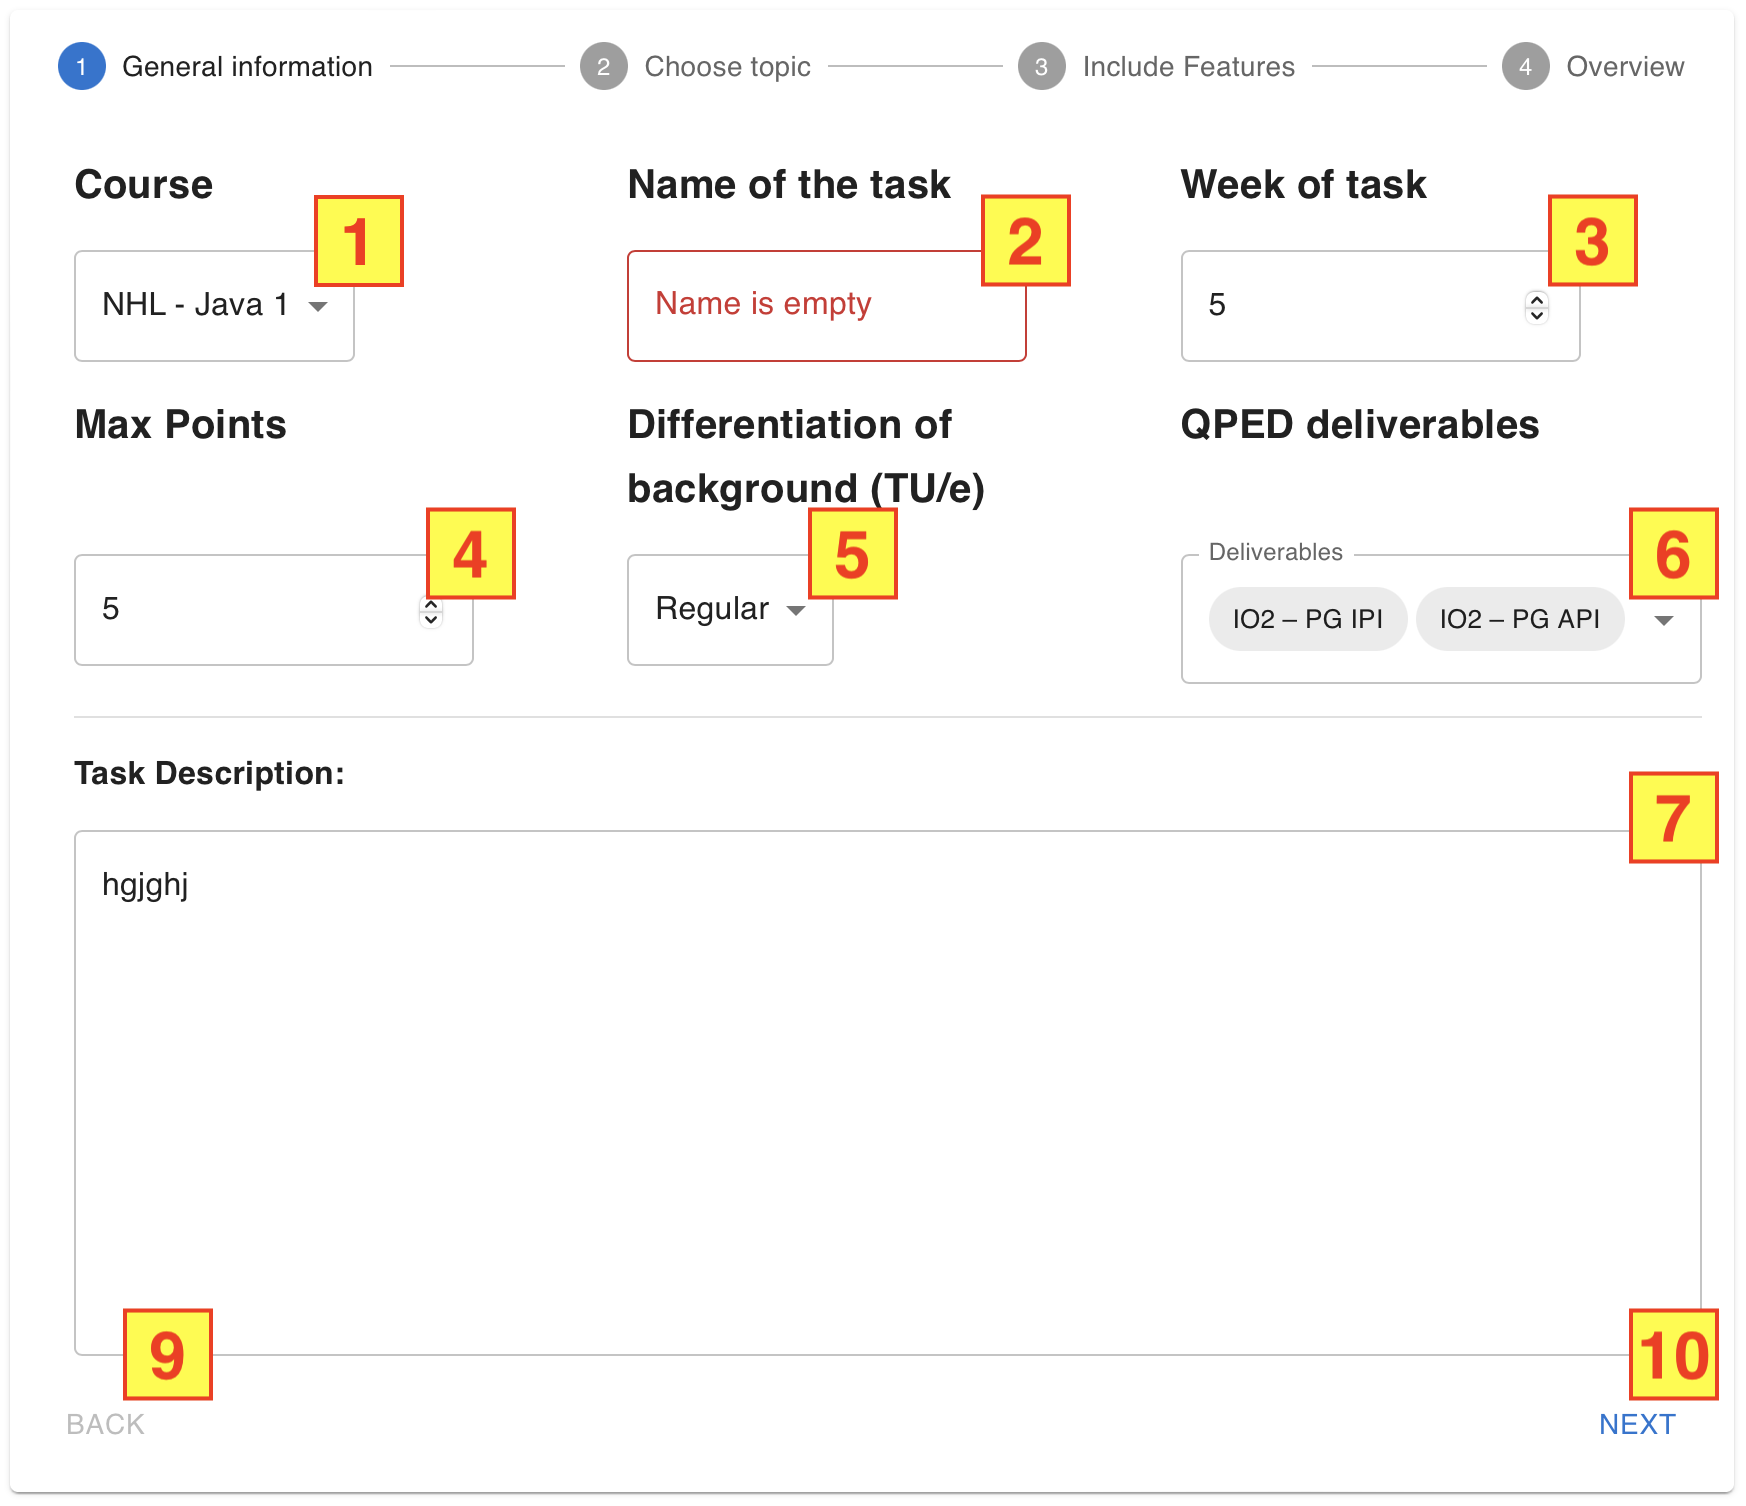
\includegraphics[width=0.8\textwidth]{figures/taskcreation1}
  \end{center}
  \caption{Step one of the \textit{task creation process}.}
  \label{fig:taskcreation1}
\end{figure}

\subsection{Meta-Information}
\label{sub:metainfo}
Specifying the meta-information for a \textit{task} is done by clicking the \textit{"Create New Task"}-Button on the \nameref{sec:home}.
The steps 1 and 2 are desgined to enter this meta-information consisting of the following parameters (marked with corresponding labels 
in Figure~\ref{fig:taskcreation1} and Figure~\ref{fig:taskcreation2}):

\begin{enumerate}
  \item \textbf{Course} \\
    Select the couse to which the assignment belongs. A dropdown provides a list of available courses.
  \item \textbf{Task Name} \\
    A name for the task. This name should \textbf{not} be empty and has to be \textbf{unique} in order to \textit{add the task} to the home screen list (Figure~\ref{fig:homescreen}, label 3). The name does not have to be unique in order to export the task as a JSON-File.
    \begin{attention}
      Only use \textbf{characters} that are \textbf{legal in file names}. The \textit{name} will be part of the exported file name.
    \end{attention}
  \item \textbf{Task Week} \\
    The week in which the task has to be solved. Also indicates the expected knowledge level of the students.
  \item \textbf{Max Points} \\
    Specify the maximum number of points that students can achieve in this \textit{task}. This is also used for computation of the final score achieved by the student, when the \textit{rubric} gets \textit{filled out}.
  \item \textbf{Differentiation of Background} \\
    Only change this value if the course is a \textit{TU/e}-course. This value corresponds to different variants of assignments.
  \item \textbf{QPED Deliverables} \\
    Select all QPED deliverables that students have used for this assignment. Either because they were used to teach the topics that are practiced by this assignment, the assignment itself uses a deliverable or students may use a deliverable to solve the assignment. 
  \item \textbf{Task Description} \\
    Used to provide a short description of the task at hand. The main purpose of this parameter is to allow the assessors of a \textit{task} to quickly verify that they are assessing the right \textit{task}.
  \item \textbf{Main Topic} \\
    Select a main topic for the \textit{task}. The available topics are nested within categories. This \textit{main topic tree} is depicted as a dropdown. In order to select a topic, you have to select a \textit{leaf node} of this tree.

\end{enumerate}

\begin{figure}[h]
  \begin{center}
    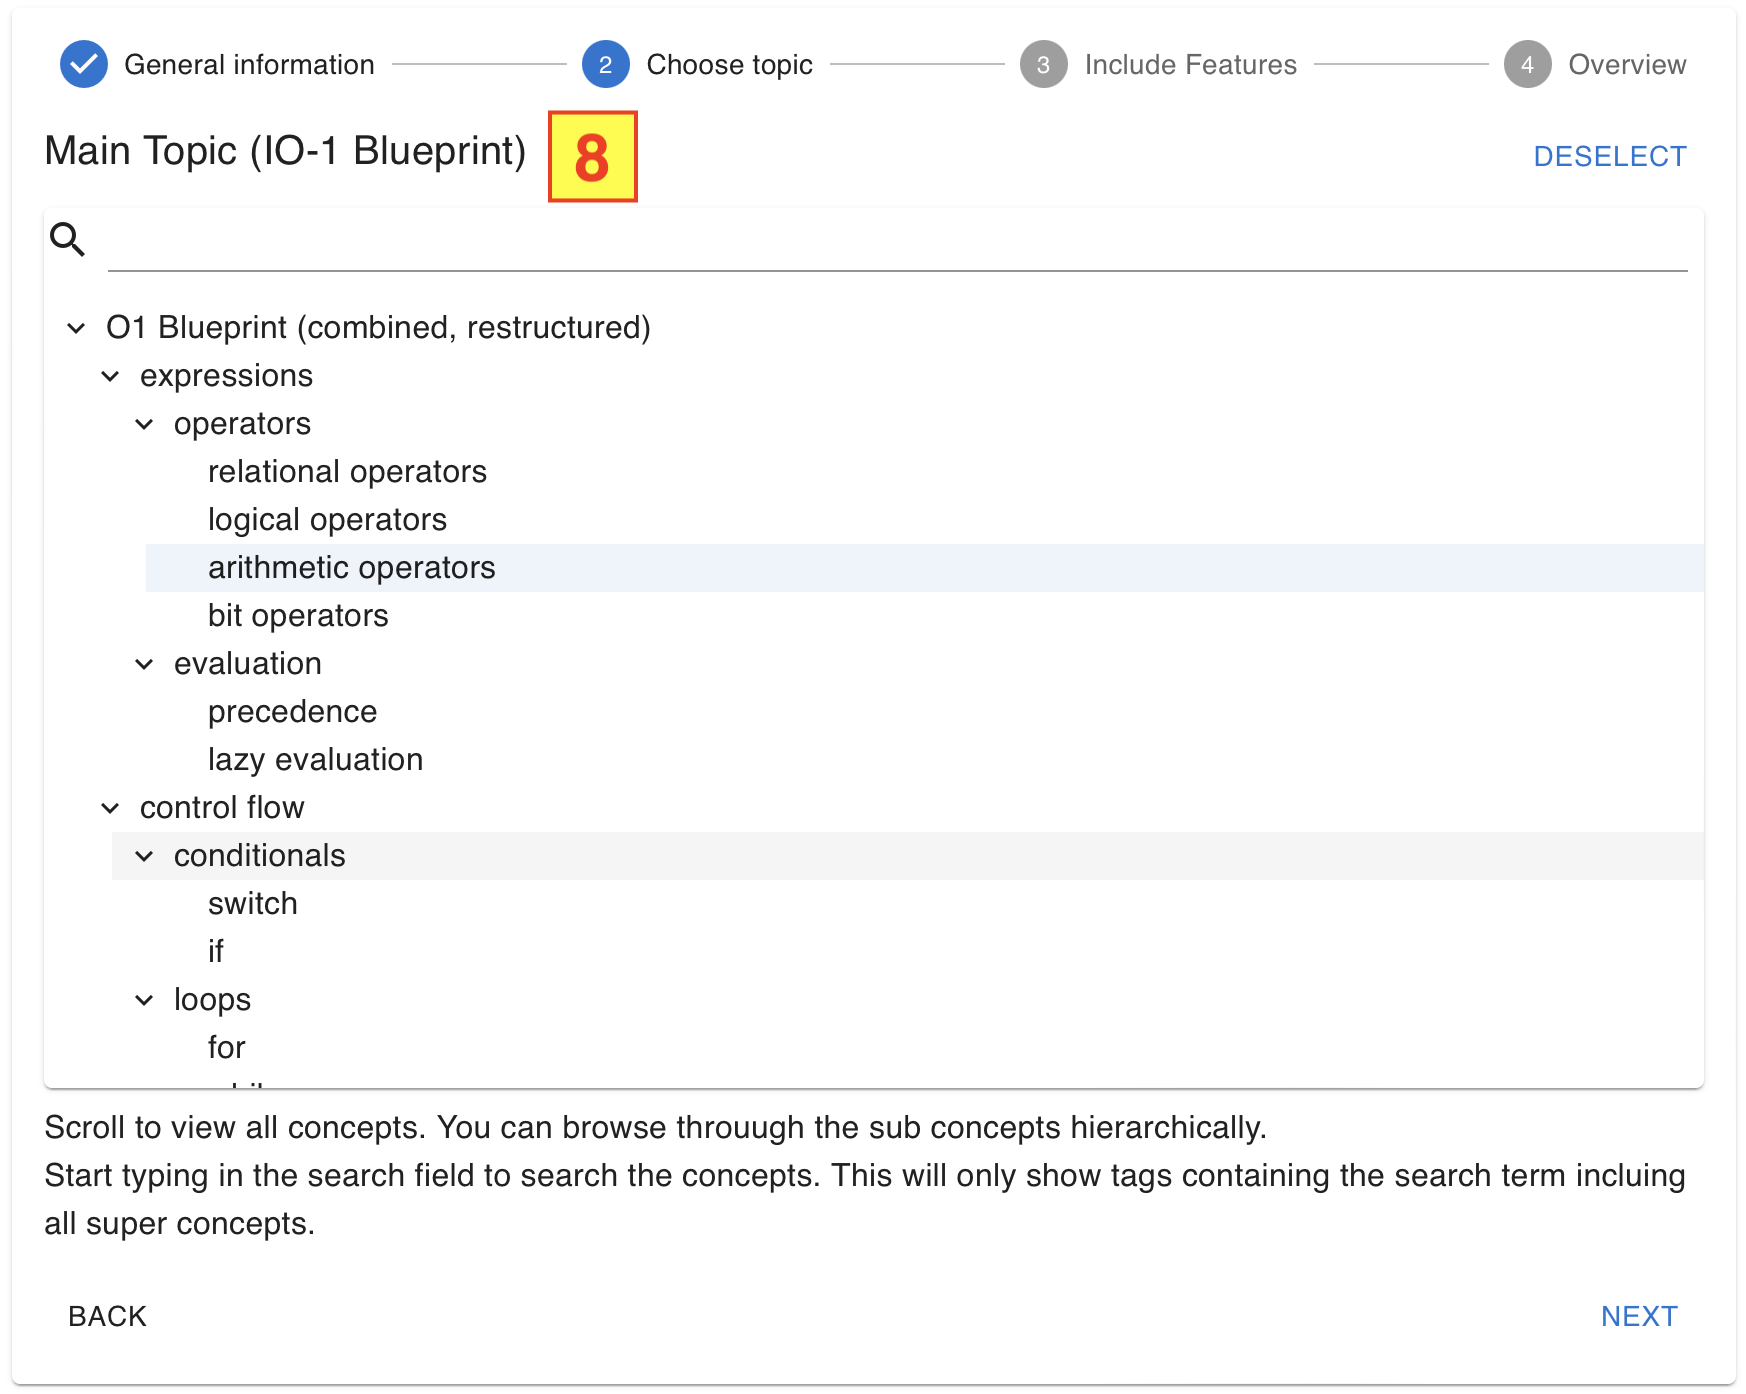
\includegraphics[width=0.8\textwidth]{figures/taskcreation2}
  \end{center}
  \caption{Step two of the \textit{task creation process}.}
  \label{fig:taskcreation2}
\end{figure}

\subsection{Features}
\label{sub:features}
Features for a \textit{task} can be selected from three main groups: \textit{Basic}, \textit{Advanced} and \textit{Procedural Guidance}.
Set a check to include the corresponding feature and chose a weight to determine how heavily the students ability to fulfill the features requirements affect their final score.

\begin{figure}[h]
  \begin{center}
    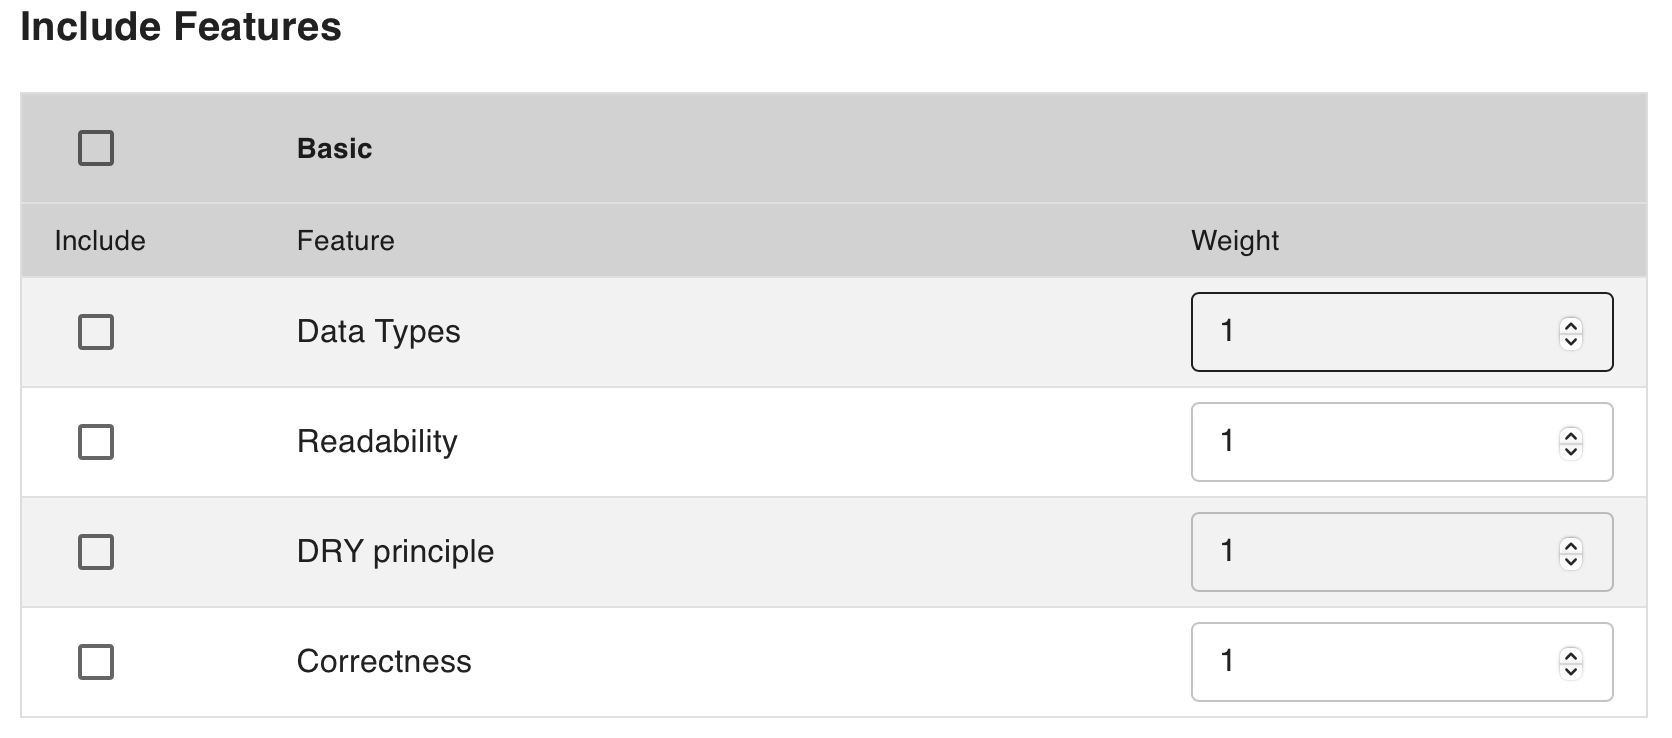
\includegraphics[width=0.95\textwidth]{figures/features}
  \end{center}
  \caption{Step three of the \textit{task creation process}.}
  \label{fig:features}
\end{figure}

\begin{wrapfigure}{r}{0.4\textwidth}
    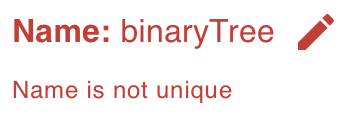
\includegraphics[width=0.3\textwidth]{figures/namenotunique}
  \caption{Case: Name is not unique.}
  \label{fig:namenotunique}
\end{wrapfigure}


\subsection{Overview}
The \textit{overview} (Figure~\ref{fig:overview}) displays all relevant information the user has entered in the process. It also notifies the user if the \textit{task name} chosen is not unique (Figure~\ref{fig:namenotunique}). In this case, the user can edited the name right in the \textit{overview} by clicking the "pen"-symbol. Furthermore, the "Add Task"-Button will be visible but not enabled while the "Export JSON"-Button will be visible regardless of whether the name is unique. After pressing each of the two buttons, the user is brought back to the \nameref{sec:home}.
The user also has the ability to add additional comments.


\begin{figure}[h]
  \begin{center}
    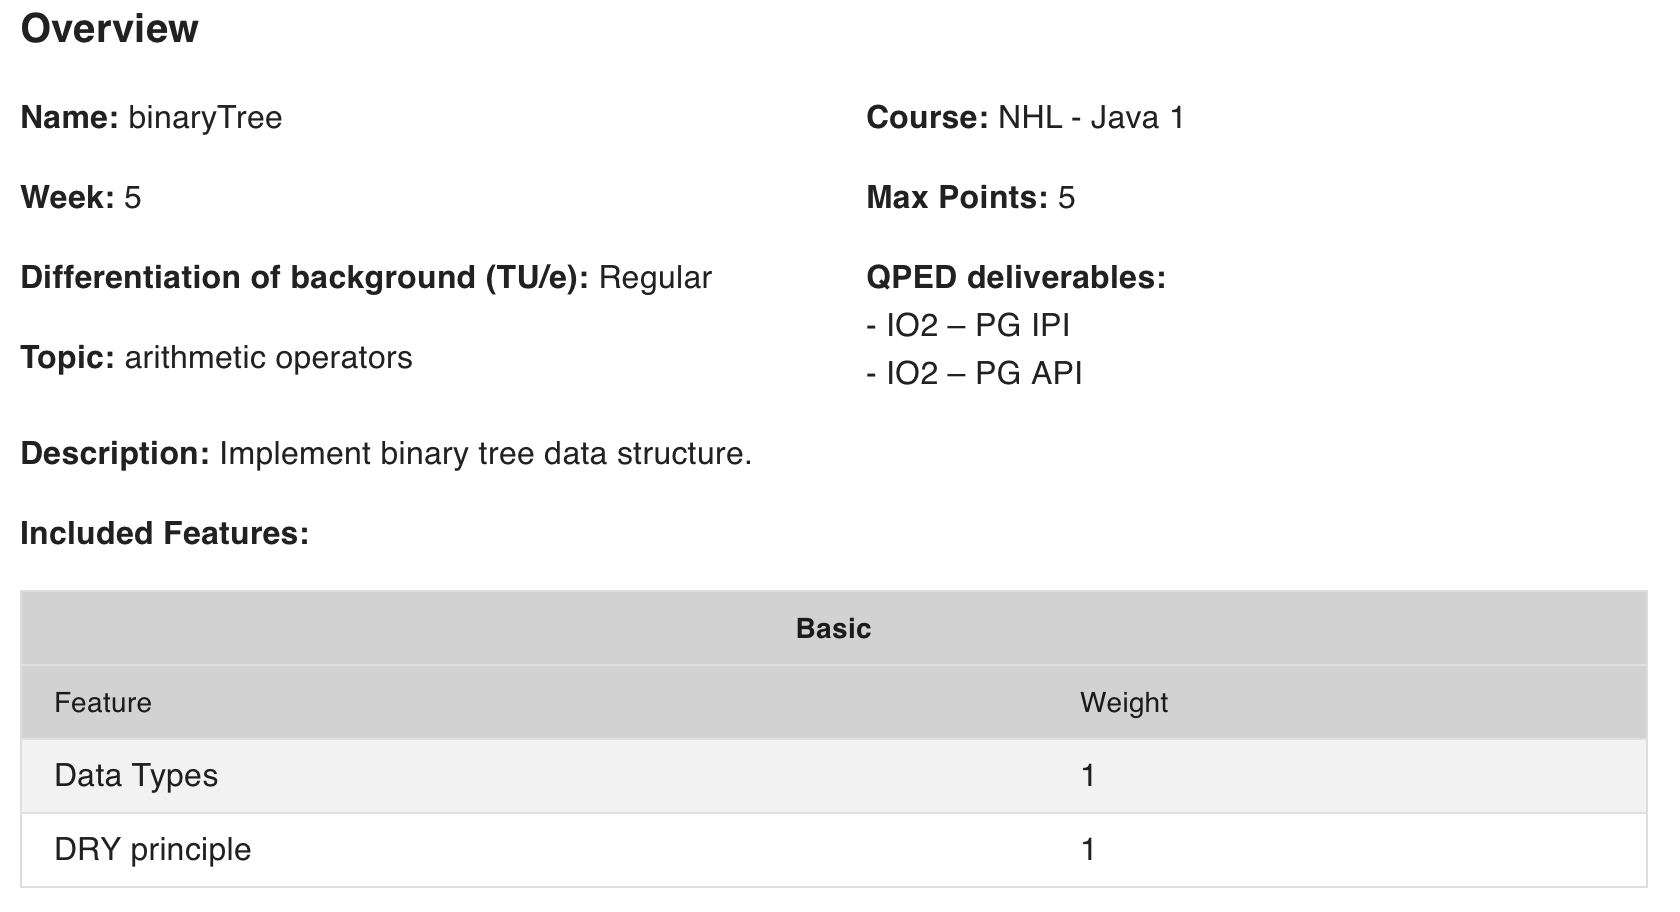
\includegraphics[width=0.6\textwidth]{figures/overview}
  \end{center}
  \caption{The final step of the \textit{task creation process}.}
  \label{fig:overview}
\end{figure}




